\documentclass{standalone}
\usepackage{tikz}
\usetikzlibrary{patterns, positioning}
\usepackage[sfdefault]{ClearSans} %% option 'sfdefault' activates Clear Sans as the default text font
\usepackage[T1]{fontenc}

\begin{document}
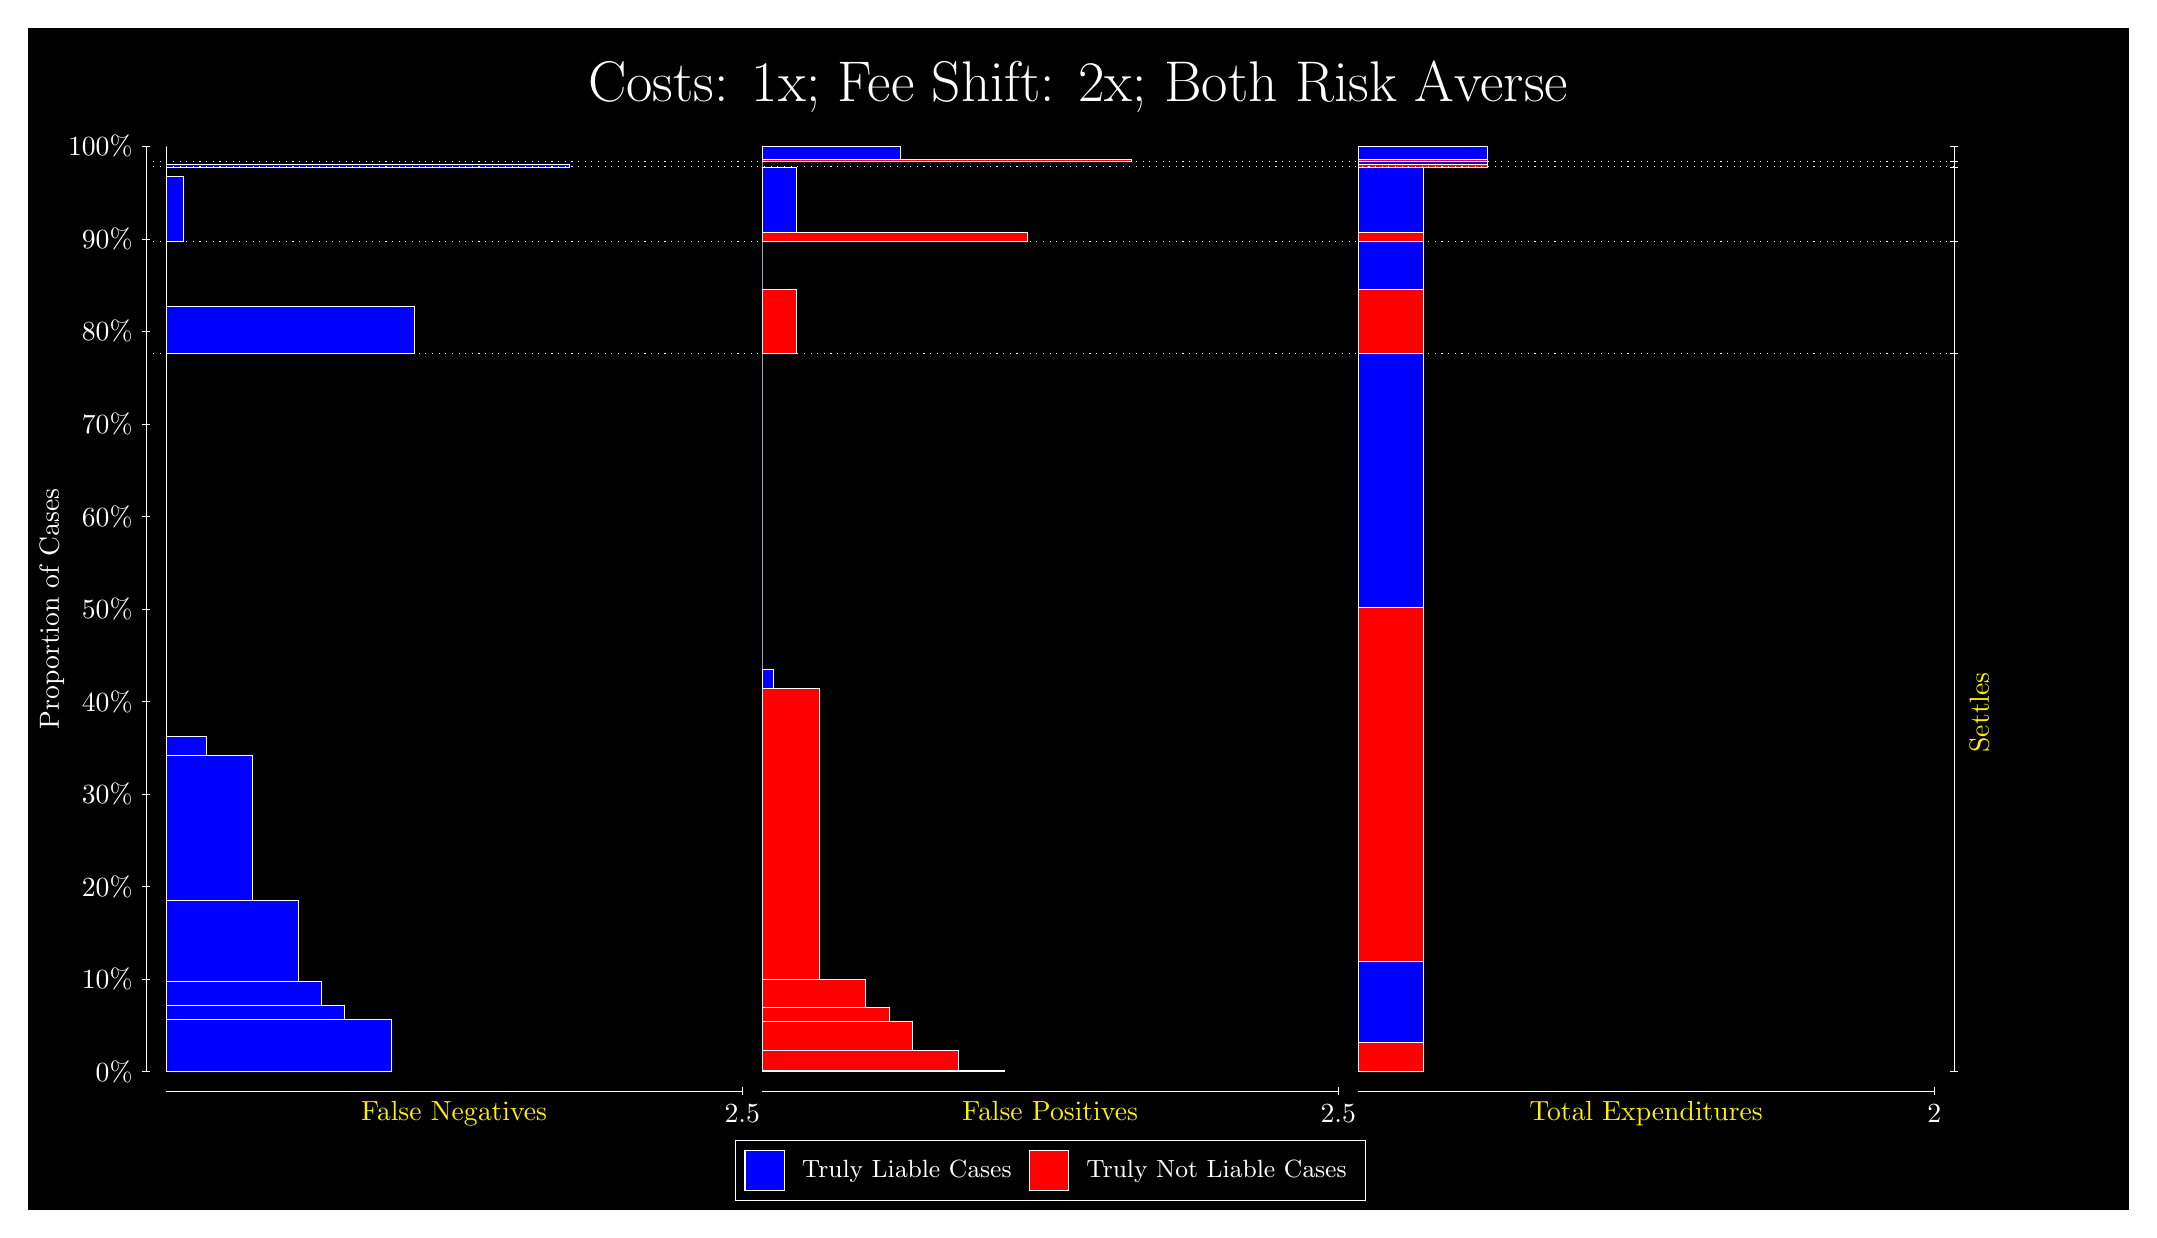
\begin{tikzpicture}
\draw[fill=black] (0,0) rectangle (26.667,15);
\draw[text=white] (0,13.5) rectangle (26.667,15) node[midway] {\huge Costs: 1x; Fee Shift: 2x; Both Risk Averse};
\draw[white, very thin] (1.5,1.75) -- (1.5,13.5);
\node[rotate=90, text=white, anchor=center] at (0.3, 7.625) {Proportion of Cases};
\draw[white, very thin] (1.45,1.75) -- (1.55,1.75);
\node[text=white, anchor=east] at (1.45, 1.75) {0\%};
\draw[white, very thin] (1.45,2.925) -- (1.55,2.925);
\node[text=white, anchor=east] at (1.45, 2.925) {10\%};
\draw[white, very thin] (1.45,4.1) -- (1.55,4.1);
\node[text=white, anchor=east] at (1.45, 4.1) {20\%};
\draw[white, very thin] (1.45,5.275) -- (1.55,5.275);
\node[text=white, anchor=east] at (1.45, 5.275) {30\%};
\draw[white, very thin] (1.45,6.45) -- (1.55,6.45);
\node[text=white, anchor=east] at (1.45, 6.45) {40\%};
\draw[white, very thin] (1.45,7.625) -- (1.55,7.625);
\node[text=white, anchor=east] at (1.45, 7.625) {50\%};
\draw[white, very thin] (1.45,8.8) -- (1.55,8.8);
\node[text=white, anchor=east] at (1.45, 8.8) {60\%};
\draw[white, very thin] (1.45,9.975) -- (1.55,9.975);
\node[text=white, anchor=east] at (1.45, 9.975) {70\%};
\draw[white, very thin] (1.45,11.15) -- (1.55,11.15);
\node[text=white, anchor=east] at (1.45, 11.15) {80\%};
\draw[white, very thin] (1.45,12.325) -- (1.55,12.325);
\node[text=white, anchor=east] at (1.45, 12.325) {90\%};
\draw[white, very thin] (1.45,13.5) -- (1.55,13.5);
\node[text=white, anchor=east] at (1.45, 13.5) {100\%};

\draw[white, very thin] (24.457,1.75) -- (24.457,13.5);
\draw[white, very thin] (24.407,1.75) -- (24.507,1.75);
\node[anchor=west] at (24.407, 1.75) {};
\draw[white, very thin] (24.407,10.874) -- (24.507,10.874);
\node[anchor=west] at (24.407, 10.874) {};
\draw[white, very thin] (24.407,12.29) -- (24.507,12.29);
\node[anchor=west] at (24.407, 12.29) {};
\draw[white, very thin] (24.407,13.239) -- (24.507,13.239);
\node[anchor=west] at (24.407, 13.239) {};
\draw[white, very thin] (24.407,13.305) -- (24.507,13.305);
\node[anchor=west] at (24.407, 13.305) {};
\draw[white, very thin] (24.407,13.5) -- (24.507,13.5);
\node[anchor=west] at (24.407, 13.5) {};

\draw[white, very thin, fill=blue] (1.75,1.75) rectangle (4.6044,2.4141);
\draw[white, very thin, fill=blue] (1.75,2.4141) rectangle (4.0188,2.5944);
\draw[white, very thin, fill=blue] (1.75,2.5944) rectangle (3.7261,2.8991);
\draw[white, very thin, fill=blue] (1.75,2.8991) rectangle (3.4333,3.9291);
\draw[white, very thin, fill=blue] (1.75,3.9291) rectangle (2.8478,5.7692);
\draw[white, very thin, fill=blue] (1.75,5.7692) rectangle (2.2623,6.0036);
\draw[white, very thin, fill=red] (1.75,6.0036) rectangle (1.75,10.874);
\draw[white, very thin, fill=blue] (1.75,10.874) rectangle (4.8971,11.474);
\draw[white, very thin, fill=red] (1.75,11.474) rectangle (1.75,12.29);
\draw[white, very thin, fill=blue] (1.75,12.29) rectangle (1.9696,13.116);
\draw[white, very thin, fill=red] (1.75,13.116) rectangle (1.75,13.239);
\draw[white, very thin, fill=blue] (1.75,13.239) rectangle (6.8732,13.275);
\draw[white, very thin, fill=red] (1.75,13.275) rectangle (1.75,13.305);
\draw[white, very thin, fill=red] (1.75,13.305) rectangle (1.75,13.341);
\draw[white, very thin, fill=blue] (1.75,13.341) rectangle (1.75,13.5);
\draw[white, very thin, fill=red] (9.3189,1.75) rectangle (12.393,1.7668);
\draw[white, very thin, fill=red] (9.3189,1.7668) rectangle (11.807,2.0201);
\draw[white, very thin, fill=red] (9.3189,2.0201) rectangle (11.222,2.3933);
\draw[white, very thin, fill=red] (9.3189,2.3933) rectangle (10.929,2.5717);
\draw[white, very thin, fill=red] (9.3189,2.5717) rectangle (10.636,2.9172);
\draw[white, very thin, fill=red] (9.3189,2.9172) rectangle (10.051,6.6201);
\draw[white, very thin, fill=blue] (9.3189,6.6201) rectangle (9.4652,6.8545);
\draw[white, very thin, fill=blue] (9.3189,6.8545) rectangle (9.3189,10.874);
\draw[white, very thin, fill=red] (9.3189,10.874) rectangle (9.758,11.689);
\draw[white, very thin, fill=blue] (9.3189,11.689) rectangle (9.3189,12.29);
\draw[white, very thin, fill=red] (9.3189,12.29) rectangle (12.686,12.413);
\draw[white, very thin, fill=blue] (9.3189,12.413) rectangle (9.758,13.239);
\draw[white, very thin, fill=red] (9.3189,13.239) rectangle (9.3189,13.269);
\draw[white, very thin, fill=blue] (9.3189,13.269) rectangle (9.3189,13.305);
\draw[white, very thin, fill=red] (9.3189,13.305) rectangle (14.003,13.341);
\draw[white, very thin, fill=blue] (9.3189,13.341) rectangle (11.075,13.5);
\draw[white, very thin, fill=red] (16.888,1.75) rectangle (17.711,2.1231);
\draw[white, very thin, fill=blue] (16.888,2.1231) rectangle (17.711,3.1531);
\draw[white, very thin, fill=red] (16.888,3.1531) rectangle (17.711,7.6501);
\draw[white, very thin, fill=blue] (16.888,7.6501) rectangle (17.711,10.874);
\draw[white, very thin, fill=red] (16.888,10.874) rectangle (17.711,11.689);
\draw[white, very thin, fill=blue] (16.888,11.689) rectangle (17.711,12.29);
\draw[white, very thin, fill=red] (16.888,12.29) rectangle (17.711,12.413);
\draw[white, very thin, fill=blue] (16.888,12.413) rectangle (17.711,13.239);
\draw[white, very thin, fill=red] (16.888,13.239) rectangle (18.534,13.269);
\draw[white, very thin, fill=blue] (16.888,13.269) rectangle (18.534,13.305);
\draw[white, very thin, fill=red] (16.888,13.305) rectangle (18.534,13.341);
\draw[white, very thin, fill=blue] (16.888,13.341) rectangle (18.534,13.5);
\draw[white, dotted] (1.5,10.874) -- (24.457,10.874);
\draw[white, dotted] (1.5,12.29) -- (24.457,12.29);
\draw[white, dotted] (1.5,13.239) -- (24.457,13.239);
\draw[white, dotted] (1.5,13.305) -- (24.457,13.305);
\draw[white, very thin] (1.75,1.5) -- (9.0689,1.5);
\node[text=yellow, anchor=north] at (5.4094, 1.5) {False Negatives};
\draw[white, very thin] (9.0689,1.45) -- (9.0689,1.55);
\node[text=white, anchor=north] at (9.0689, 1.45) {2.5};

\draw[white, very thin] (9.3189,1.5) -- (16.638,1.5);
\node[text=yellow, anchor=north] at (12.978, 1.5) {False Positives};
\draw[white, very thin] (16.638,1.45) -- (16.638,1.55);
\node[text=white, anchor=north] at (16.638, 1.45) {2.5};

\draw[white, very thin] (16.888,1.5) -- (24.207,1.5);
\node[text=yellow, anchor=north] at (20.547, 1.5) {Total Expenditures};
\draw[white, very thin] (24.207,1.45) -- (24.207,1.55);
\node[text=white, anchor=north] at (24.207, 1.45) {2};

\node[text=yellow, centered, rotate=90] at (24.777, 6.3118) {Settles};





\draw (12.978300999999998,1.5) node[draw=none] (baseCoordinate) {};
\begin{scope}[align=center]
        \matrix[scale=0.5, draw=white, below=0.5cm of baseCoordinate, nodes={draw}, column sep=0.1cm]{
            \node[rectangle, draw, minimum width=0.5cm, minimum height=0.5cm, fill=blue] {}; &
            \node[draw=none, font=\small, text=white] (B) {Truly Liable Cases}; &
            \node[rectangle, draw, minimum width=0.5cm, minimum height=0.5cm, fill=red] {}; &
            \node[draw=none, font=\small, text=white] (B) {Truly Not Liable Cases}; \\
            };
\end{scope}

\end{tikzpicture}
\end{document}